% \pdfminorversion=4
%\documentclass[letterpaper, 10 pt, conference]{IEEEtran}
\documentclass{article}



\usepackage{cite}
\usepackage{graphicx}
\usepackage{subcaption}
\usepackage{amsmath}
\usepackage{amssymb}
\usepackage{amsthm}
\usepackage{algorithmic,algorithm}
\usepackage{array}
\usepackage{hyperref}
\usepackage{url}
\usepackage{bm}
\usepackage{subcaption}

\usepackage{nccmath,mathtools}

\linespread{0.95}

\let\labelindent\relax
\usepackage{enumitem}
\setlist{leftmargin=0pt,itemindent=15pt,labelwidth=8pt,labelsep=7pt,listparindent=15pt,topsep=2pt, itemsep = 2pt}

\usepackage{xcolor,comment}

\newtheorem{proposition}{Proposition}%[section]
\newtheorem{theorem}{Theorem}%[section]
\newtheorem{lemma}{Lemma}%[section]
\newtheorem{corollary}{Corollary}%[section]
\newtheorem{assumption}{Assumption}%[section]

\theoremstyle{definition}
\newtheorem{definition}{Definition}%[section]

\theoremstyle{remark}
\newtheorem{remark}{Remark}%[section]

\newcommand{\pp}[2]{\frac{\partial #1}{\partial #2}}

\newcommand{\tr}{\operatorname{Tr}}


\newcommand{\yhat}{ \hat{\textbf{y}}_{t|t-1}}
\newcommand{\qhatpre}{\hat{q}_{t|t-1}}
\newcommand{\qhatpost}{\hat{q}_{t|t}}
\newcommand{\tC}{\tilde{C}_t}


\begin{document}
	\title{\LARGE \bf Safe Learning Documentation}
	\author{Tianpeng Zhang}
	\maketitle
	
	\section{Introduction}
	This is the documentation of the Python implementation of the Safe Learning algorithm and its related simulations based on \cite{li2021safe}. The code can be found in the following online GitHub repository: \url{https://github.com/lina-robotics-lab/SafeLearning}. 
	
	See Section \ref{sec:system} for a mathematical description about the system model we used in the simulations.
	
	See Section \ref{sec:howto} for a quick guide to run the simulation.
	
	Section \ref{sec:details} contains detailed documentations for each component of the implementation.
	
	\section{System Model}\label{sec:system}
	We consider a dampened spring-mass system in the simulation. The system contains a mass with weight $m>0$ attached to a spring with stiffness constant $k>0$. The mass is restricted to move along a one-dimensional surface perpendicular to the gravity direction. We assume no friction between the mass and the surface, but there is a drag negatively proportional to the velocity of the mass, with a drag constant $\lambda>0$. We can apply an external force
	$u$ on the mass along the trajectory of its movement to control its state.
	
	Let $x\in \mathbb{R}$ be the location of the mass, the system equation in continuous time can be defined as 
	\begin{equation}\label{eq:contModel}
		\ddot{x} = (-k x - \lambda \dot{x} + u)/m
	\end{equation}

	In the implementation, we approximate \eqref{eq:contModel} using a discrete-time system defined by 
	\begin{equation}\label{eq:discModel}
		s_t : = \begin{bmatrix}
			x_t\\
			v_t
		\end{bmatrix} = (\begin{bmatrix}
		0& \Delta \\
		- \frac{k \Delta}{m}  & - \frac{\lambda \Delta}{m} 
	\end{bmatrix}+I)\begin{bmatrix}
	x_{t-1}\\
	v_{t-1}
	\end{bmatrix}  + \begin{bmatrix}
	0\\
	\frac{\Delta}{m}
	\end{bmatrix}u_{t-1}
	\end{equation}
where $s_t$ is the system state at time step $t$, and $\Delta>0$ is a small constant representing the sampling time interval.

	\section{How to run the simulations}\label{sec:howto}

	\textbf{Step 1}: clone the git repository to a local folder by 
	\begin{verbatim}
		git clone https://github.com/lina-robotics-lab/SafeLearning
	\end{verbatim}

	\textbf{Step 2}: Install the Python packages required by the simulation. 
	Especially, jupyterlab, matplotlib, scipy, and cvxpy.
	
	I recommend installing the Python environment manager called $conda$ \url{https://docs.conda.io/en/latest/miniconda.html}, and follow \url{https://docs.conda.io/projects/conda/en/latest/user-guide/tasks/manage-environments.html} to create a new Python environment. This ensures the new packages do not interfere with the original Python on your computer which serves crucial purposes such as rendering your desktop and windows.
	
	A typical flow of operations after installing \textit{conda} is
	\begin{verbatim}
		conda create -n SafeLearningEnv python=3.9 scipy jupyterlab matplotlib
		conda activate SafeLearningEnv 
		pip install cvxpy
	\end{verbatim}
	
	\textbf{Step 3}: Ensure the Python environment we created in Step 2 in command prompt by 
	\begin{verbatim}
		conda activte SafeLearningEnv
	\end{verbatim}
	Navigate to the SafeLearning folder in command prompt. Then start the jupyter lab by running
	\begin{verbatim}
		jupyter lab
	\end{verbatim}
	The default browser of your computer should pop up and show a tab loading the jupyter lab. Eventually you will see something like the screenshot in Figure \ref{fig:jupyter}.
	\begin{figure}[h]
		\centering
		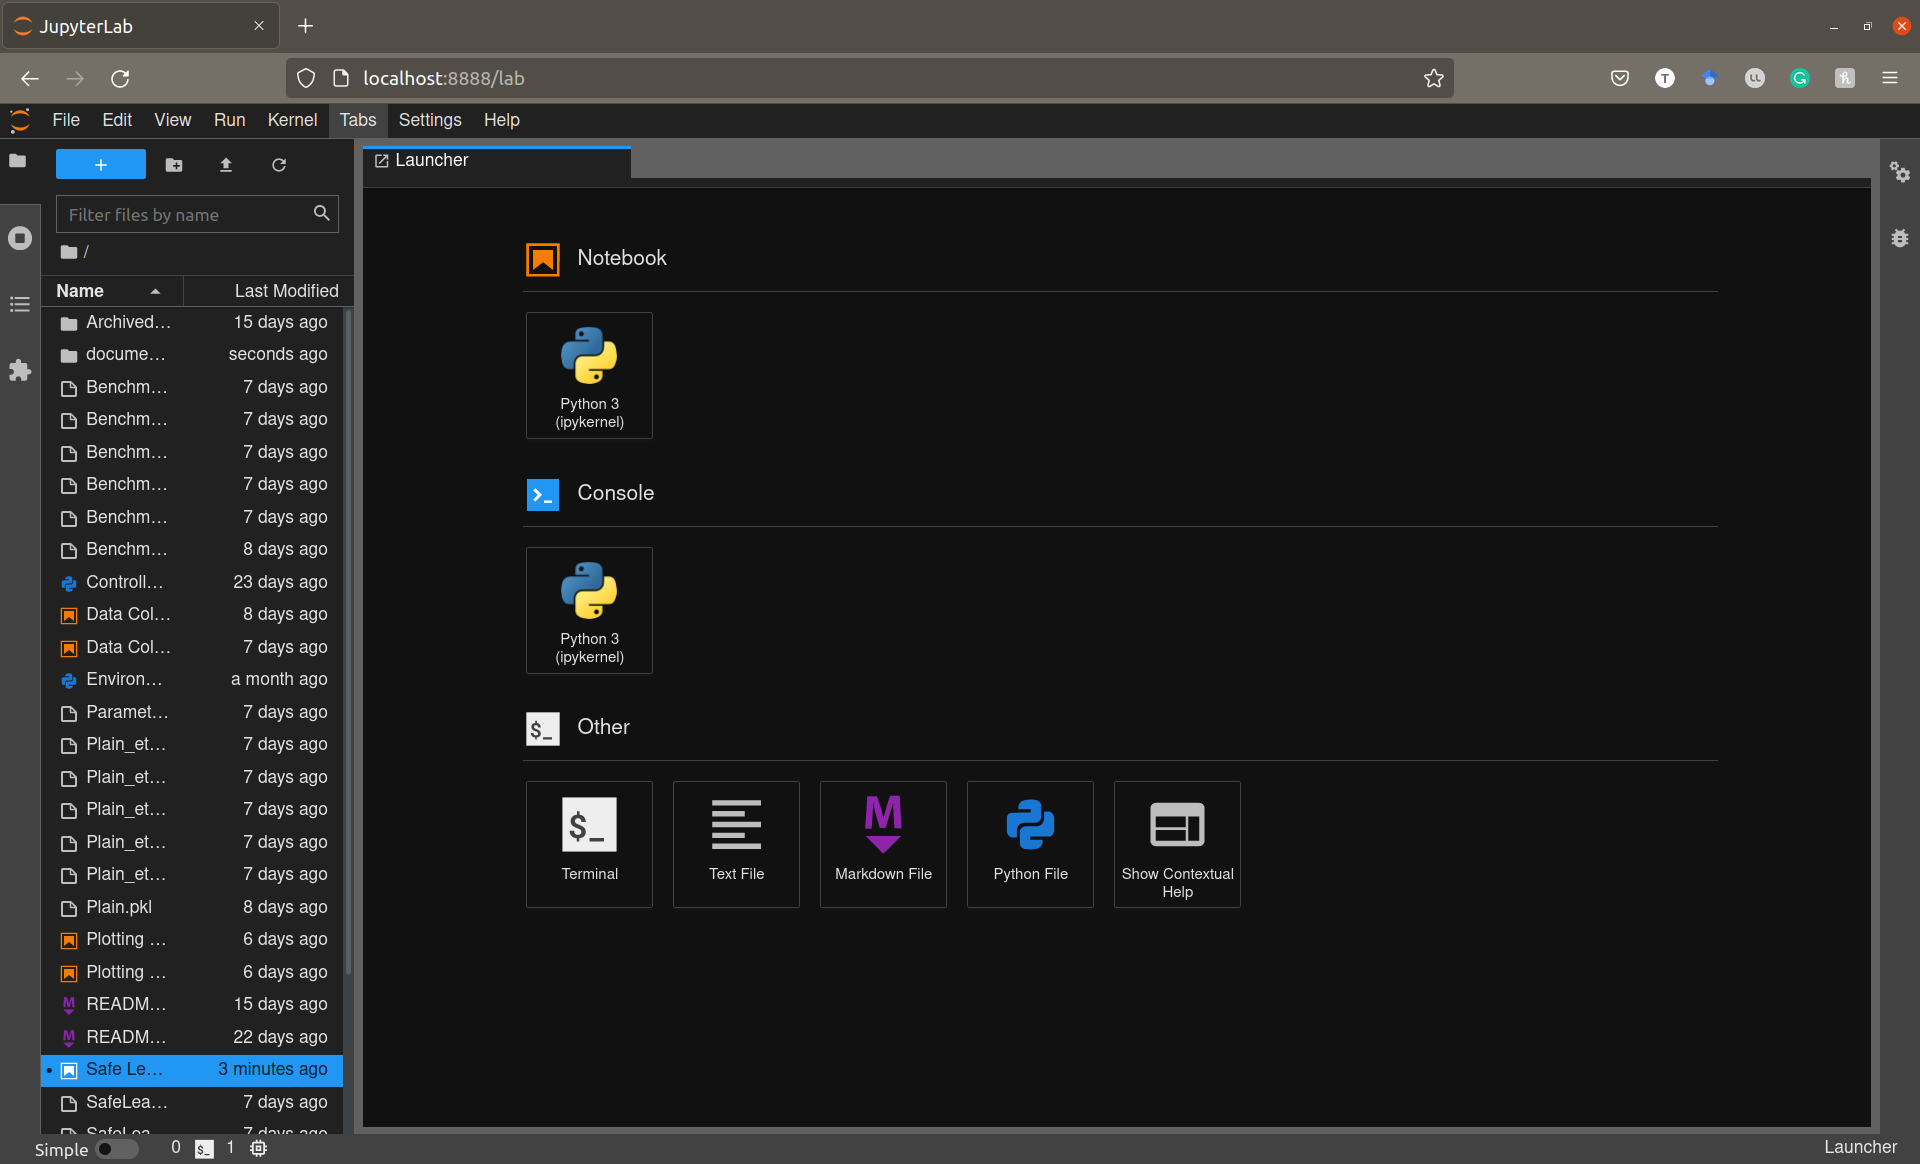
\includegraphics[width=0.8\linewidth]{jupyter}
		\caption{}
		\label{fig:jupyter}
	\end{figure}
	
	\textbf{Step 4}: in the jupyter lab window, navigate to \textit{notebooks} foler, double click to open the \textit{[Safe Learning Simulation.ipynb]} notebook. 
	
	Press \textit{Esc} to enter command mode. 
	
	Press \textit{Ctrl+a} to select all cells.
	
	Finally, press \textit{Ctrl + enter} to run the entire notebook from start to end.
	
	The Python notebook works similarly as the live scripts/run by section utility in Matlab. Watch this video for a 30-min beginner's tutorial on Python notebooks:\url{https://www.youtube.com/watch?v=HW29067qVWk}.
	
	\section{Detailed Documentations}\label{sec:details}
	\subsection{File Structure}
	The repository is structured in the following manner:
	
	\begin{verbatim}
		Repository Root
		- Scripts(.py files) and README
		- documentation
		  - Latex files
		- notebooks
		  - Demonstration notebook(SafeLearningSimulation.ipynb)
		  - Devel
		    - Notebooks under development
		    - The data folder
		      - Data files(.pkl)
		  - Folders containing specific experiments
		    - The simulation notebook
		    - The plotting notebook
		    - The data folder
		      - Data files(.pkl)
	\end{verbatim}
	We ensure the data files are encapsulated in the inner-most layer and the scripts are exposed in the outer-most layer, and that folders for individual experiments follow the template specified above.
	\subsection{Environment}
	\subsection{Controllers}
	\subsection{Subroutines}
	\subsection{Simulations}
	\bibliographystyle{IEEEtran}
	\bibliography{reference}
\end{document}